This term is originated in the digital media industry near the year 2008
 \cite{DefineGamefication} to summarise the use of game elements on other
contexts. An example of this are education, sales and marketing. 

Gamification was widespread between the years 2008 and 2010. The use of 
this idea grew exponencially from the use on banners for marketing to be implemented
on big educational solution now a days.

This idea initially was use on the 80s to make an upgrade to a gametype called MUD
\emph{Multy User Dungeons}. The person behind this was Richard Bartle who begin to
analise the people who played this games and found 4 stereotypes of players,\ref{fig:Players}.
With this types of players he made a new kind of MUD to satisfy each type of player. After this
people began to use this to engage to people and capture their attention. 

\begin{figure}[!htb]
  \centering
  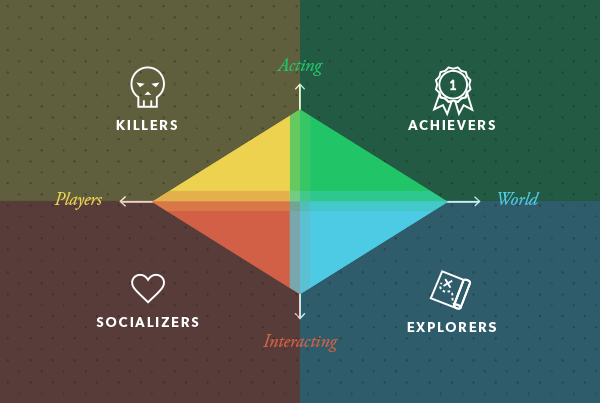
\includegraphics[width=0.5\textwidth]{images/TypeOfPlayersBartle.png}
  \caption[Caption for LOF]{Real caption\footnotemark}
  \label{fig:Players}
\end{figure}

\footnotetext{Source: \url{http://www.example.com/theimage.png}}
 	

Nowadays Gamification has become a really useful tool to engage people. With this in mind
the industry and people using it needs a description to unite all diferent concepts
about Gamification so everyone can understand it and begin to work with a unique conception.
Gamificaton is \emph{the use of game design elements in non-game related contexts}. 
Within the definition are four concepts that are very important to understand.

\begin{itemize}

\item Game:

\item Element:

\item Design:

\item Non-Game Context:

\end{itemize}

Gamification can be use on multiple context where the attention of the user is needed. Some of this context are education, sales and marketing.

\begin{itemize}

\item Education: In this context the use of gamification can be seen in different ideas to engage the
the students and keep them interested. Some of this concepts can be use in schools and universities
where the students are 

\item Sales and marketing:

\end{itemize}

